\documentclass[border = 5pt, tikz]{standalone}

\usepackage{tikz}
\usepackage{tikz-qtree}
\usetikzlibrary{trees} % this is to allow the fork right path

\begin{document}

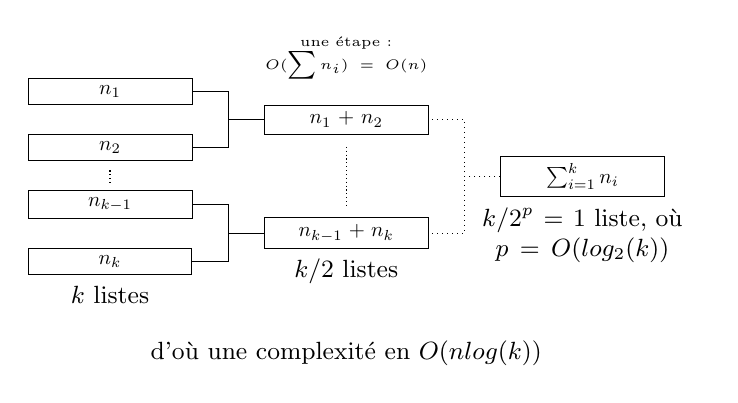
\begin{tikzpicture}[level distance=4cm,sibling distance=0.5cm,scale=.75]
\tikzset{edge from parent/.style= 
            {draw,
                edge from parent fork left},every tree node/.style={draw,minimum width=2cm,text width=1in, align=center},grow'=left}
\Tree 
    [. {$ \sum_{i=1}^{k} n_i $}
        \edge[dotted];
        [. {$ n_{k-1} + n_k $}
            [.{$n_k$} ]
            [.{$n_{k-1}$} ]
        ]
        \edge[dotted];
        [. {$n_1 + n_2$}
            [.{$n_2$} ]
            [.{$n_1$} ]
        ]
    ]
\node[font=\small] at (-8, -2) {$k$ listes};
\node[font=\small] at (-4, -1.6) {$k/2$ listes};
\node[text width=3cm, font=\small, align=center] at (0, -1) {$k/2^p = 1$ liste, où $p = O(log_2(k))$};
\node[font=\small] at (-4, -3) {d'où une complexité en $O(nlog(k))$};
\node[text width=3cm, font=\tiny, align=center] at (-4, 2) {une étape : $O(\sum n_i) = O(n)$};
\draw[densely dotted] (-4,0.5) -- (-4,-0.5);
\draw[densely dotted] (-8,0.1) -- (-8,-0.1);
\end{tikzpicture}
\end{document}